\documentclass[12 pt, a4paper]{article}


%\usepackage[titlepage]{polytechnique}
\usepackage{polytechnique}

\usepackage{graphicx}		% inclure des graphiques
\usepackage{hyperref}			% lien hypertexte
\usepackage{array}   % pour faire des tableaux
\usepackage{pict2e}  % pour faire des figures géomètriques
\usepackage[utf8]{inputenc}		% reconnaître les caractères spéciaux
\usepackage[T1]{fontenc}		% polices de caractère
\usepackage[french]{babel}	% utiliser les régles d'affichage françaises
\usepackage{lmodern}

% Package Lu
\usepackage[centertags]{amsmath}
\usepackage{amsfonts}
\usepackage{amssymb}
\usepackage{amsthm}
\usepackage{amsmath}
\usepackage{graphicx}

\usepackage{pstricks-add}
	
% pour les notes de bas de page
\AddThinSpaceBeforeFootnotes % à insérer si on utilise \usepackage[french]{babel}
\FrenchFootnotes % à insérer si on utilise \usepackage[french]{babel}

% Section counter ???
% \setcounter{section}{1}
% \renewcommand\thesection{\arabic {section}}
% \renewcommand\thesection{\Roman {section}}



\title[Data camp 2018]{Data camp Lab6}
\subtitle{Hyperparameters tuning on SVM models}
\author{Lu \textsc{Lin}, Olivier \textsc{Coudray}}
\date{16 février 2018}

\begin{document}

\maketitle




\begin{abstract}
Ce dossier contient un sous-dossiers nommé \texttt{DFO\_src} et ....

\end{abstract}

\section{Introduction}
Dans ce rapport nous allons tester quatre algorithmes d'optimisation de type boîte-noire pour calibrer les hyperparamètres de l'algorithme de \textit{Support Vector Machine} (SVM) appliqué à notre problème de classification : \textit{Random Search}, \textit{BO (Optimisation bayésienne)} de \texttt{scikit-learn}, \textit{CMA-ES} et \textit{DFO-TR}. L'objectif est de tester la performance de ces algorithmes d'optimisation dans un cas pratique. L'objectif n'est donc pas de résoudre directement notre problème mais de trouver la meilleure façon de le résoudre. Nous comparons les résultats obtenus avec le fameux problème de classification MNIST (Lab2 du Data Camp) en tenant compte des spécificités du SVM. Ici, nous considérons uniquement l'algorithme SVC avec le noyau gaussien de \texttt{scikit-learn}. Ainsi, la dimension de l'espace de recherche est 2 ($\gamma$ et $C$). Sachant que ces deux paramètres sont strictement positifs d'échelles différentes, nous opérons une transformation (logarithmique/affine)\footnote{Comme ce qu'on faisait pour le Lab2.} pour ramener l'espace de recherche à $[-5, 5]^{D}$\footnote{$D$ étant la dimension de l'espace. Ici $D=2$.} comme celui de la plate-forme COCO. Nous montrons que cette transformation revient à diminuer le conditionnement (\textit{condition number} $\kappa$) et rendre les solvers efficaces. Il est à remarquer que, sans cela, certains solvers seront incapable de fonctionner.


\section{Description des données}
\subsection{MNIST}
Il s'agit d'un problème de classification de 10 classes (les chiffres manuscrit de 0 à 9) avec les 70000 images de taille $28\cdot 28$ (dont 60000 pour le train set et 10000 pour le test set).

\subsection{Speech recognition}
Nous avons réduit notre problème de classification original de Kaggle de 30 classes à 11 classes. Il s'agit de classifier les mots à partir du son prononcé par un humain de durée environ 1 seconde. Ce sont des vocabulaires anglais simples, comme "yes", "no", "up", "down", "left", "right", "on", "off", "stop", "go" et les autres.



\section{Pré-traitement des données (Preprocessing)}
\subsection{MNIST}
Pour le problème MNIST, le seul pré-traitement est la normalisation des images. Il s'agit de diviser chaque pixel par 255 pour que les valeurs soient comprises entre 0 et 1. Faisons une remarque sur lien entre la normalisation et le paramètre $\gamma$ en résumant le rapport de Lab2\footnote{Veuillez trouver une explication plus complète dans le rapport Lab2 de Lu Lin.}. En fait, la normalisation ici n'est pas obligatoire, mais elle a un impact direct sur la valeur du paramètre $\gamma$. En regardant la formule du noyau gaussien~(\ref{kernel}), on déduit que si on multiplie chaque pixel par $10$, il faut diviser $\gamma$ par $10^{2}$ et garder la même constante $C$ pour avoir la même précision (aka accuracy). Cela a été confirmé numériquement. 

\begin{equation}\label{kernel}
k(x_{i}, x_{j}) = e^{-\gamma \| x_{i}- x_{j} \|^{2}} = e^{-\gamma^{\prime} \| x_{i}^{\prime}-x_{j}^{\prime}\|^{2}}
\end{equation}

Dans la section \ref{results}, nous allons analyser la structure des données en utilisant cette remarque.

\subsection{Speech recognition}

Le pré-traitement des enregistrements audio s'est fait en deux étapes. Dans un premier temps, il s'agit de recouper les extraits audio de façon à ne sélectionner que la partie où le mot est prononcé. Plus concrètement, on passe un filtre sur le signal pour couper tous les sons en deçà d'un certain seuil d'intensité (dans notre cas 15 dB). Dans un deuxième temps (c'est la partie la plus importante), il faut extraire les données de l'enregistrement. La technique standard consiste à considérer le spectrogramme de l'extrait audio. Dans le cadre de la reconnaissance vocale, il est conseillé d'utiliser un spectrogramme légèrement différent (échelle non linéaire en fréquence) : \textit{Mel-frequency cepstrum}.

Notons que l'on peut considérer ou du moins visualiser ces spectrogrammes comme des images (matrices). A titre d'exemple, on peut observer ci-dessous, les spectrogrammes Mel pour deux mots différents.

\begin{figure}
   \begin{minipage}[c]{.46\linewidth}
      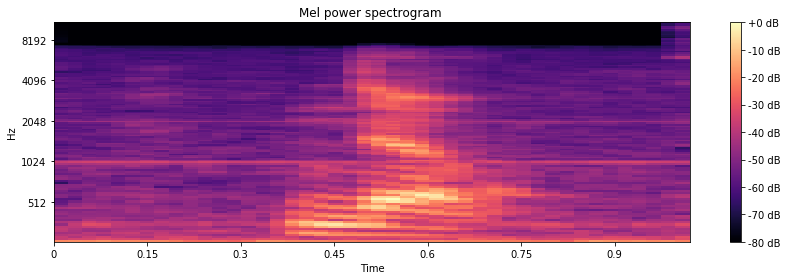
\includegraphics[scale=0.39]{no1.png}
      \caption{"No"}   
     \end{minipage} \hfill
   \begin{minipage}[c]{.46\linewidth}
      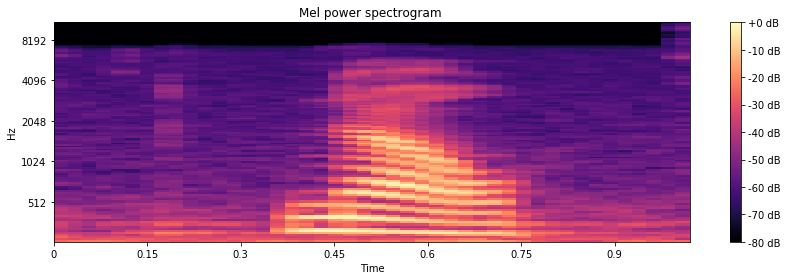
\includegraphics[scale=0.39]{no2.png}
      \caption{"No"}  
   \end{minipage}
\end{figure}

\begin{figure}
   \begin{minipage}[c]{.46\linewidth}
      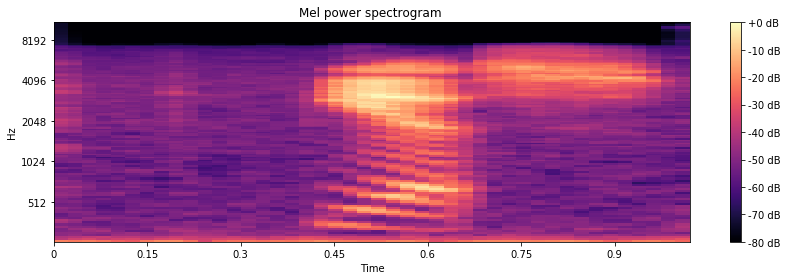
\includegraphics[scale=0.39]{yes1.png}
      \caption{"Yes"}   
     \end{minipage} \hfill
   \begin{minipage}[c]{.46\linewidth}
      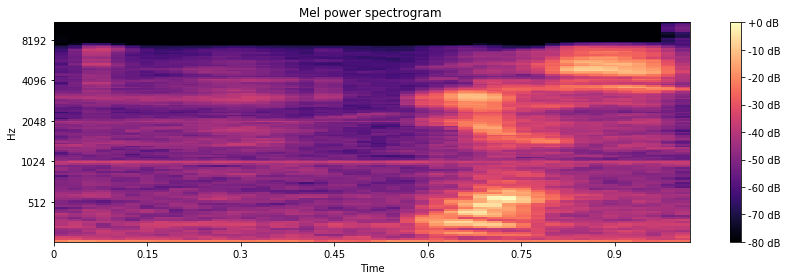
\includegraphics[scale=0.39]{yes2.png}
      \caption{"Yes"}  
   \end{minipage}
\end{figure}

\paragraph{Remarque}
\textbf{Lu}: Est-ce que cela tu pourrais compléter cette partie avec le pre-processing que t'as fait ? On pourrait mettre quelques images de spectrogramme. Par exemple, deux spectrogramme similaires de "go" et un spectrogramme très différent (comme celui de "yes" ou autres ?). Cela permet de leur convaincre que le spectrogramme suffit pour classifier ces mots.


\section{Transformation de l'espace de recherche}\label{transform}
Remarquons que pour la machine SVM avec le noyau gaussien, les deux paramètres $\gamma$ et $C$ n'ont pas ni les même sensibilités (l'échelle), ni le domaine de recherche. Par exemple, pour le MNIST, les paramètres state-of-the-art sont $\gamma = 0.025$, $C = 10$ \cite{results}. D'après les résultats du Lab2, le paramètre $C$ pourrait s'élever à l'ordre de 1000, alors que étant contraint par l'exponentiel du noyau gaussien, le résultat est sensible à la valeur de $\gamma$. D'où l'idée de faire au moins une transformation affine. Nous montrons que cela revient à diminuer le conditionnement dans un cas simple. Considérons la fonction ellipsoïde en dimension 2 suivante. 

\begin{equation*}
\frac{x^2}{a^2} + \frac{y^2}{b^2} = 1
\end{equation*}
Si $a>b$, alors le conditionnement $\kappa = (\frac{a}{b})^2$. Il est facile de vérifier que si on fait une transformation affine sur $y$ pour le ramener au même l'ordre de grandeur, on diminue $\kappa$, ainsi on simplifie le problème. La Figure~(\ref{fig:step}) explique pourquoi DFO-TR peut-être fortement influencé par ce genre de transformation. Remarquons que les paramètres de DFO-TR qu'on a choisi sont adapté pour la plate-forme COCO, c'est à dire que la zone de recherche est inclue dans $[-5,5]^{D}$. Ici, la fonction Step est quasiment plat (constant) dans cette zone et que le minimum se trouve à la frontière. Or, la stratégie de DFO-TR consiste faire une grid-search avec $2D+1$ points dans la phase initiale\footnote{En partant de zéro, ce grid-search consiste à évaluer les points en perturbant une coordonnée à chaque fois i.e. $(x_{1}+\delta, \ldots)$, $(x_{1}-\delta, \ldots)$, $(x_{1}, x_{2}+\delta, \ldots)$ ...etc.}, en plus la taille de \textit{delta} initiale $\Delta_{0}$ qu'on avait choisi empêche l'évaluation de dehors de $[-5,5]^{D}$. Tout cela entraîne l'échec de DFO-TR.

\begin{figure}[h]
\centering
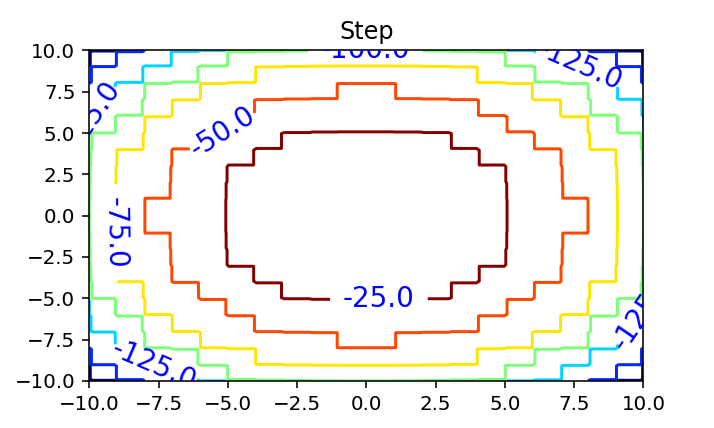
\includegraphics[width = 0.5\textwidth]{Step_function_inverse.png}
\caption{Step function inverse}
\label{fig:step}
\end{figure}

\subsection{Handle the boundary}
Dans notre problème 

\paragraph*{TODO Lu} Je vais le faire. 



 % le couple $\gamma = 0.0242$, $C = 632.65$ 

\section{Commentaires et les résultats}\label{results}

\subsection{MNIST}

De nos expériences dans le Lab2, DFO-TR converge au bout de $10$ à $30$ évaluations. Et les précisions obtenues sont supérieurs à $98\%$. Le tableau suivant illustre les minima locaux trouvés:

\begin{center}
\begin{tabular}{|c|c|c|c|}
  \hline
  % after \\: \hline or \cline{col1-col2} \cline{col3-col4} ...
  $\gamma$ & $C$ & $\text{size}=7000$ & $\text{size}=70000$ \\
  $0.0413$ & $78.22$ & $0.973$ & $0.9851$ \\
  $0.0242$ & $632.65$ & $0.971$ & $0.9848$ \\
  $0.02845$ & $521.6$ & $0.967$ & $0.985$ \\
  $0.024$ & $100$ & $0.963$ & $0.9864$ \\
  \hline
\end{tabular}
\end{center}
Nous avons échantillonné $7000$ images parmi $70000$ pour le hyperparamters tuning. Nous entraînons SVM sur $6000$ images et testons sur $1000$ images. Les valeurs dans les deux dernières colonnes représentent les précisions sur le \emph{test set}.

\textbf{Remarque}: \textit{Scikit-Learn} a mélangé le \emph{train set} et \emph{test set} de MNIST. Donc, c'est normal d'avoir des précisions légèrement différentes par rapport aux données de \textit{Keras}.

\subsection*{Speech recognition}

Dans le traitement des données audio, on sépare le jeu de données en trois datasets : un d'entraînement, un de validation et un de test. Pour des raisons de complexité et de temps de calcul, on ne réalise l'entraînement que sur $1600$ données dans cette étude comparative. La validation se fait sur un ensemble de $400$ extraits audio.

Dans le cas de DFO-TR et CMA-ES, on note le nombre d'appels à la fonction d'évaluation ainsi que le temps d'exécution global. Dans le cas de \textit{Random Search} et BO, on fixe au départ un budget de $100$ évaluations et on note le temps d'exécution.

\begin{center}
\begin{tabular}{|c|c|c|c|c|c|}
  \hline
  % after \\: \hline or \cline{col1-col2} \cline{col3-col4} ...
  $\text{Optimizer}$ & $\gamma$ & $C$ & $\text{Score}$ & $\text{time (sec)}$ & $\text{n eval}$ \\
  \hline
  $\text{DFO-TR}$ & $5.75$ & $774$ & $0.823$ & $553$ & $35$ \\
  $\text{CMA-ES}$ & $10.18$ & $745$ & $0.823$ & $4865$ & $288$\\
  $\text{Random Search}$ & $10.61$ & $946$ & $0.820$ & $1560$ & $100$\\
  $\text{BO}$ & $6.31$ & $500$ & $0.820$ & $1794$ & $100$\\
  \hline
\end{tabular}
\end{center}

L'étude montre que l'algorithme DFO-TR est le plus efficace aussi bien du point de vue de l'optimum trouvé mais également et surtout du point de vue du temps de calcul.

L'algorithme CMA-ES, en dépit du temps de calcul important fournit des renseignements intéressant sur la fonction de coût (voir graphe suivant). En particulier, on vérifie que la fonction est séparable.

\begin{figure}[h]
\centering
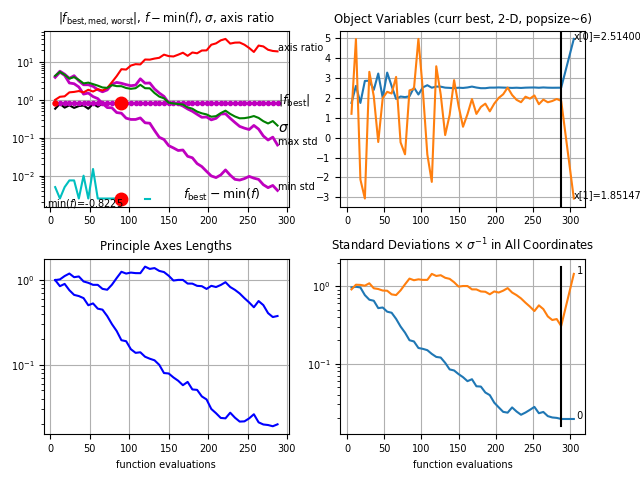
\includegraphics[width = 0.5\textwidth]{CMA_plot.png}
\caption{CMA-ES plot}
\label{fig:step}
\end{figure}

\quad

\bibliographystyle{plain}
\bibliography{references}

\end{document} 